\begin{figure}[H]
\centering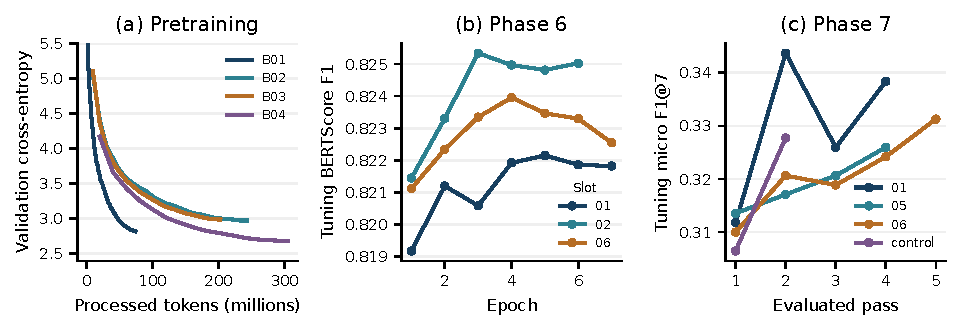
\includegraphics[width=\textwidth]{figures/learning_curves.pdf}
\caption{Saved learning curves. Pretraining protocols differ across bases, and the first plot displays loss below 5.5 for readability. Task curves show evaluated checkpoints; slot05 retrieval is incomplete in the archived run.}
\label{fig:curves}
\end{figure}

The lowest logged foundation losses are 2.82046, 2.97407, 2.98855 and 2.68014 for bases~01--04. Several task runs peak before their last epoch. The full retrieval model is best at pass~2, and the small KD advantage at pass~1 reverses at pass~2. Summarization gains are also small on the score scale. These curves explain why retaining the best checkpoint matters: a lower final training loss or a longer run does not guarantee a better submission.

\section{Error Analysis and Discussion}
\subsection{Phase-wise failure modes}
NER errors are concentrated in participant and witness spans. In the selected hybrid OOF predictions, APP has 76 true positives out of 407 gold entities and 342 predictions; RESP has 71 out of 381 gold and 376 predictions. Their F1 scores are 0.20294 and 0.18758, compared with 0.95907 for DATE. Only 111/407 APP and 122/381 RESP gold spans appear among the exact candidates. This puts a clear limit on threshold tuning: it cannot recover a span that is missing from the candidate set. The aggregate counts do not show the precise legal context behind each error.

Role prediction has a different problem: rare labels have very little independent support. All overruled-precedent examples come from one document. HighF1 raw decoding scores 0.42415 on document OOF and 0.53335 on dev when only supported labels are averaged; its fixed all-thirteen dev score is 0.45130. Pair corrections slightly improve supported dev F1 but lower OOF F1 to 0.42156, and CRF variants also trail raw OOF. This is a reason to be cautious about a small dev improvement.

The selected judgment model misses 502 positive outcomes and makes 355 false-positive predictions. Positive recall is 0.71412, compared with 0.79703 for the negative class. Chunk sampling could omit outcome-bearing text, but that explanation was not checked through manual examples. Duplicates and unfinished outer folds also limit the conclusion. In statutes, slot~01 predicts 4.92 labels per case against 3.68 gold, with subset accuracy 0.04143. Distillation reduces the predicted count to 4.80 and raises subset accuracy to 0.04515, with micro F1 0.47888. Both models still overpredict; calibration alone does not solve the long tail.

The summarization audit records 5,430 truncated fitting targets for base~03. Its audit outputs average 398.18 words, while references average 858.93, so a good embedding score can still hide missing content. Retrieval also has a structural limit: ten training queries have no relevant case, while others have more than seven. Even a perfect dev ranking can reach only 0.61812 under the seven-output rule. The neural views cover only part of very long candidates, although full-document BM25 still has access to their words.
